\chapter{Purpose}
\label{chap:purpose}

As was mentioned in Chapter \ref{chap:intro}, Custos aims to solve the
cryptographic key storage problem, making encryption easier to use and
an available option for securing user data across a range of modern
use cases. To accomplish this goal, Custos must be both usable and
secure.  Furthermore, it must be flexible enough to overcome existing
hurdles to utilizing encryption in modern situations.

In this chapter, we'll discusses the goals Custos hopes to achieve, a
number of possible application where Custos can make encryption a more
usable primitive, and the threat model that Custos aims to defend
against.

\section{Goals}

Custos's primary goal is as stated above: ``To solve existing key
storage challenges and make encryption more easily utilized to secure
modern data storage paradigms''. To achieve this goal, Custos aims
to provide the basis of a Key Storage as a Service architecture. This,
in turn, entails a handful of sub-goals. If we decompose the core
Custos goal stated previously into it's primary components, we get:

\begin{packed_desc}
\item[Provide Key Storage:] ``To solve existing \emph{key storage}
  challenges...''
\item[Easily Usable:] ``...and make encryption more \emph{easily
  utilized}...''
\item[Secure:] ``...to \emph{secure} modern data storage paradigms.''
\end{packed_desc}

We'll discuss the sub-goals in each of these ares in the sections below.

\subsection{Key Storage}

Custos is a type of key:value store. As such, it had better be cable
of storing key:value pairs. I expect must Custos implementations
(including the ones described in this document) to defer the actual
key:value storage aspect of Custos to existing key:value storage
systems. Why reinvent the wheel? Instead, we must identify what
aspects of key:value storage capabilities are desirable in a Custos
back end. The primary drivers of this analysis are the type of data
Custos will store, and the methods in which this data will be
accessed. We already know that Custos will primary be used to store
key:value pairs mapping data identifiers (the keys) to corresponding
encryption keys (the values). As far as accessing this data goes, we
would expect access patterns similar to that of the encrypted data
that Custos is being used to protect. Most modern data, including the
personal data that we'd expect users to use encryption and Custos to
protect, follows an append-only, read-heavy
workload~\cite{Ghemawat2003}.

With these thoughts in mind, I propose the filling as desirable traits
for a the key:value storage components of Custos.

\begin{packed_desc}
\item[Fast Access] \hfill \\ A user will likely not accept too much
  overhead having to wait on Custos when wishing to access their
  encrypted data. Thus, Custos should strive to provide quick access
  to key:value pairs. If a compromise must be made between read and
  write speed, read speed should be favored since reads will likely
  outnumber writes.
\item[Versioned Data] \hfill \\ When data is updated, it is likely
  that the user may wish to re-encrypt it with a new key (more on this
  in later sections). As such, Custos should support storing multiple
  versions of the value associated with a given key.
\item[Arbitrary Data] \hfill \\ Encryption keys come in a variety of
  shapes, sizes, and formats. To support the maximum range of
  encryption systems, Custos should allow the storage of arbitrary
  binary data associated with a given UUID key.
\end{packed_desc}

\subsection{Usability}

As we discussed in Chapter \ref{chap:intro}, Custos aims to achieve
usability across three discreet usage types: the usability of
encryption system leveraging Custos (end-user usability), the
usability of Custos to access control mechanisms (administrative
usability), and the ease with which Custos can be interfaced with
other systems (developer usability).

On the end user usability front, Custos aims to expand the
accessibility of encryption systems be providing flexibility. It aims
to provide a more natural match between desired uses for cryptography
and attainable uses of cryptography, narrowing the intention vs
capability divide. As such, Custos aims to enable encryption system to
support the following attributes of successful modern storage systems.

\begin{packed_desc}
\item[Multi-Device Support] \hfill \\ Today a given users tends to
  have multiple computing devises. And they expect to by able to sync
  their data across these devices and access it from each regardless
  of whether or not it is encrypted. Thus, Custos must support this
  form of multi-device access where the data may be decrypted and read
  from a device other than the one on which it was originally
  encrypted.
\item[Multi-User Support] \hfill \\ We like to share. User's today
  expect to be able to share files or data with their friends or
  coworkers and access data others have shared with them. Custos must
  support the ability to share encrypted files with other users,
  granting the necessary users access to the corresponding encryption
  keys so that they might decrypt and access the shared data.
\item[Flexible Protection Semantics] \hfill \\ Some data requires only
  cursory protections and should allow wide ranging access, other data
  requires moderate protection but should still allow access by a
  large group of Friends. Still other data should never be accessed by
  anyone other than its creator. Custos must support a range of
  security levels, allowing the user to select the appropriate point
  on the security burden vs accessibly risk gradient.
\end{packed_desc}

In addition to end-user usability, Custos also aims for administrative
usability, making it easy to control access to one;s data. Custos aims
to achieve this goal by providing users with the ability to grant
access on the basis of a variety of authentication parameters,
creating a flexible and straightforward system for controlling access
to encryption keys, and by proxy, the data they protect. The following
characteristics will help ensure Custos remains usable form an
administrative perspective.

\begin{packed_desc}
\item[Flexible Authentication Mechanisms] \hfill \\ Some data need
  only be protected by a simple check of what IP address wishes to
  access it, other data requires an interactive password prompt to
  access, still other data access may require a password prompt and
  multi-factor device like a cell phone. Users should be able to
  select how their data is protected and what hurdles must be jumped
  to access it.
\item[Simple Access Granting] \hfill \\ The semantics for granting a
  specific actor access to specific data for a specific capability
  should be simple and straightforward. It should be clear how to
  grant access, what level of security that access entails, and what
  the grantee is able to do with such access.
\item[Simple Access Revocation] \hfill \\ Occasionally, you will need
  to revoke access that has been previously granted. Doing so should
  be simple and have well defined semantics to ensure the user knows
  what effect revoking access is guaranteed or not guaranteed to have.
\end{packed_desc}

The final component of Custos usability is its developer usability. If
we are to expect Custos to be integrated into existing cryptographic
products, it must be easy for developers to accomplish this
feat. Custos aims to maintain a high degree of developer usability via
the following features.

\begin{packed_desc}
\item[Well Defined API] \hfill \\ Custos will expose a standard API
  for data access and a standard API for administrative
  management. These APIs will provide a well defined interface for
  interacting with a Custos server.
\item[Standard Design Patterns] \hfill \\ The Custos API will attempt
  to follow standard web-based design patterns by following a
  REST-based architecture. This bring all of the standard usability
  benefits of RESTful systems (statelessness, etc) while also being a
  well understood architecture to develop against.
\item[Standard Data Formats] \hfill \\ Custos aims to support
  arbitrary data storage. But it will do so using commonly deployed
  data standards like JSON and Base64 encoding. Their a variety of
  libraries available to deal with these formats, making it easy to
  convert between Custos API messages and native internal data types
  for a client system.
\end{packed_desc}

\subsection{Security}

Being a secure key-values tore means that Custos must be... secure.
In addition to the increased security through increased usability
items discussed above, what does it mean to be a secure key value
store? Does it mean that the key:value pairs are stored in a manner to
ensure they remain secure in the event of a server breach? Does it
mean that the server operator has no ability to access key:value pairs
directly. Does it merely mean the access to key:value pairs is well
controlled?

We discuss Custos's security models in details later in this chapter,
but Custos adopts the last of the previous questions as the basis for
it's definition of a secure key:value store. A key value storage is
secure if access to key:value pairs is well regulated. To achieve this
level regulation, Custos requires several traits:

\begin{packed_desc}
\item[Secure Communication Primitives] \hfill \\ The Custos API must
  be protected against eavesdropping and Man-In-The-Middle attack
  es. Custos leverages SSL and the existing PKI systems to achieve
  these security.
\item[Access Control] \hfill \\ Custos provides the ability to
  regulate key access in a variety of flexible means (see above). It
  provides access control at the create, read, and modify levels, and
  provides support for versioning and revocation.
\item[Access Auditing] \hfill \\ Custos logs access to all key:value
  pairs, including successful and failed attempts. This allows the
  user to view a record of who has had access to what version of a
  specific key, proving the basis for damage assessment and revocation
  analysis.
\end{packed_desc}

In addition to these times, a Custos server should also follow best
practices to avoid compromise. A full list of standard server security
techniques is outside the scope of this paper, but standard industry
practices like securing physical access, keep software up to date, and
using proper firewalls and server access controls all apply. Custos is
only as secure as the server running it (details on this point and the
full Custos threat model is discussed below).

\section{Applications}

Custos's flexibility makes it appropriate for a wide range of
application. In this section, we'll focus on several applications
domains where we feel Custos's could have the greatest impact. These
domains exhibit the ideal trifecta of Custos-suitability:

\begin{packed_item}
\item Features offered by these applications are desirable and relevant
  to modern users
\item Users could more effectively protect their data by leveraging
  these applications features in conjunction with easily usable,
  manageable, encryption.
\item Existing implementations are challenging to protect with traditional
  encryption while also remaining easily usable.
\end{packed_item}

\subsection{File Systems}

Modern file systems come in many shapes and sizes. But to most users,
they are transparent systems through with files are stored on a range
of Medea from hard drives to flash sticks to optical disks. In
addition to their role in storing user data, modern file systems often
support features like multi-user access and data sharing, multi-device
syncing, redundancy, and backup. The file system layer is the
primary entry point to user-stored data. As such, providing a usable
method for protecting file system data via strong encrypting is highly
desirable. Such protections would help users in the event of the loss
or theft of their devices, or in the event the forced confiscation of
their devices.

\begin{figure}[!tb]
  \begin{center}
    \begin{subfigure}{\textwidth}
      \begin{center}
        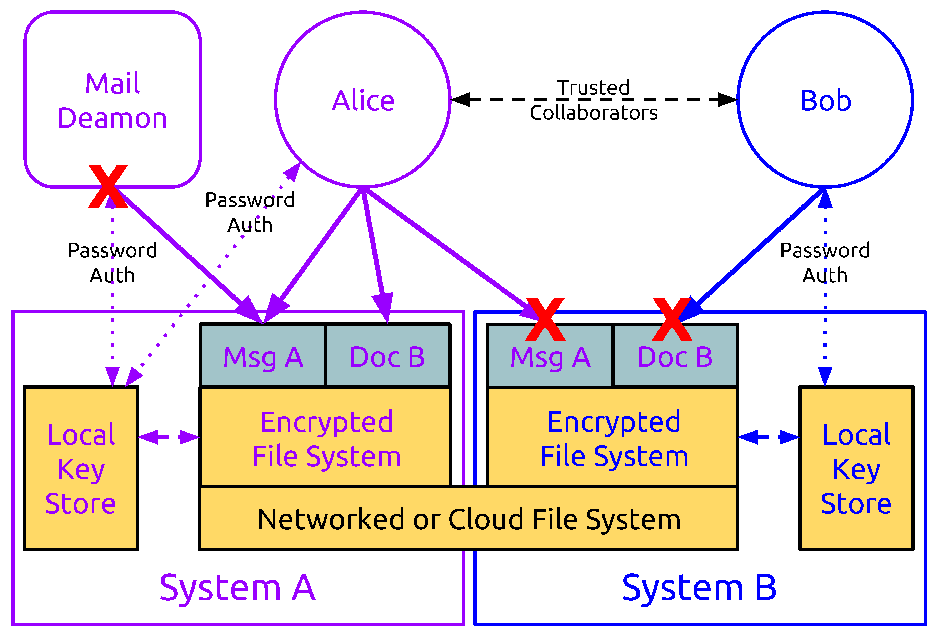
\includegraphics[width=.5\linewidth]
                        {./figs/pdf/FS-Traditional-Layered.pdf}
        \caption{Traditional Layered File System Encryption}
        \label{fig:FS-traditional-layered}
      \end{center}
    \end{subfigure}
    \begin{subfigure}{\textwidth}
      \begin{center}
        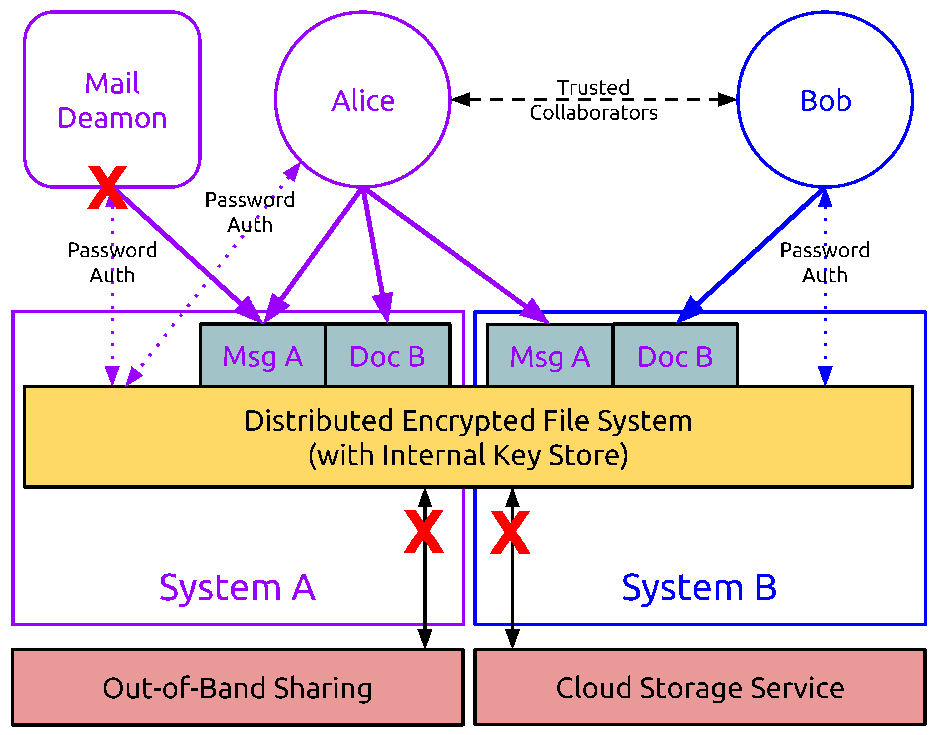
\includegraphics[width=.5\linewidth]
                        {./figs/pdf/FS-Traditional-Integrated.pdf}
        \caption{Traditional Integrated File System Encryption}
        \label{fig:FS-traditional-integrated}
      \end{center}
    \end{subfigure}
  \end{center}
  \caption{Traditional File System Encryption Challenges}
  \label{fig:FS-traditional}
\end{figure}

Unfortunately, existing encrypted file systems fail to provide
encryption in a flexible manner appropriately matched to the ways in
which users expect to utilize them. Layered encryption solutions like
dm-crypt~\cite{dm-crypt} and eCryptfs~\cite{eCryptfs, Halcrow} suffer
from a number of limitations related to their tightly-coupled local
key storage and access management components. As Figure
\ref{fig:FS-traditional-layered} shows, these systems work fine for an
individual user like Alice wishing to secure items like her mail or
documents and access them from a single machine. But they quickly
break down when trying to move beyond the simple single-user,
single-device use case. Alice can not access her encrypted mail file
across a networked file system from System B since System B has no
access to the encryption keys stored on System A. Furthermore, she can
not share a work document with a trusted collaborator like Bob, since
Bob neither has access to her encryption keys stored on System A nor
the password required to unlock these keys. A non-interactive process
like the Mail Daemon is also unable to leverage these encrypted file
systems due to the inability of such services to securely and
interactively provide a password to unlock the keys needed to decrypt
local files.

While full stack distributed encrypted file systems such as
OceanStore~\cite{Kubiatowicz2000}, Plutus~\cite{Kallahalla2003},
Cumulus4j~\cite{cumulus4j}, or Tahoe~\cite{Wilcox-O'Hearn2008} tend to
succeed in solving some of the sharing and distribution problems
inherent in local secure file systems, they still lack the flexibility
required to address the full range of desired use cases. Figure
\ref{fig:FS-traditional-integrated} shows some of the remaining issues
inherent in distributed solutions. Notably, while multi-user use cases
are better supported, non-interactive use cases are still a
challenge. Furthermore, full stack distributed file systems tend to be
wedded with specific storage systems and thus lack support for
Cloud-based Storage as a Service offerings or alternate underlying
storage technologies. These systems also lack support for most forms
of ``out-of-band'' file sharing (via e-mail, USB flash drives, etc)
due to the inability of actors outside of the integrated stack to
access the necessary encryption keys.

\begin{figure}[!tb]
  \begin{center}
    \begin{subfigure}{\textwidth}
      \begin{center}
        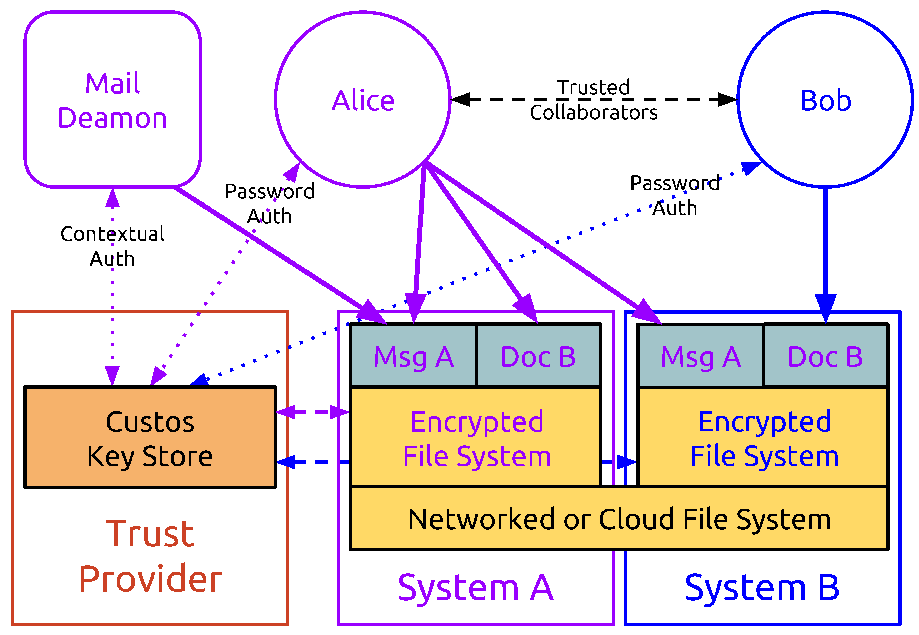
\includegraphics[width=.5\linewidth]
                        {./figs/pdf/FS-Custos-Layered.pdf}
        \caption{Layered File System Encryption with Custos}
        \label{fig:FS-custos-layered}
      \end{center}
    \end{subfigure}
    \begin{subfigure}{\textwidth}
      \begin{center}
        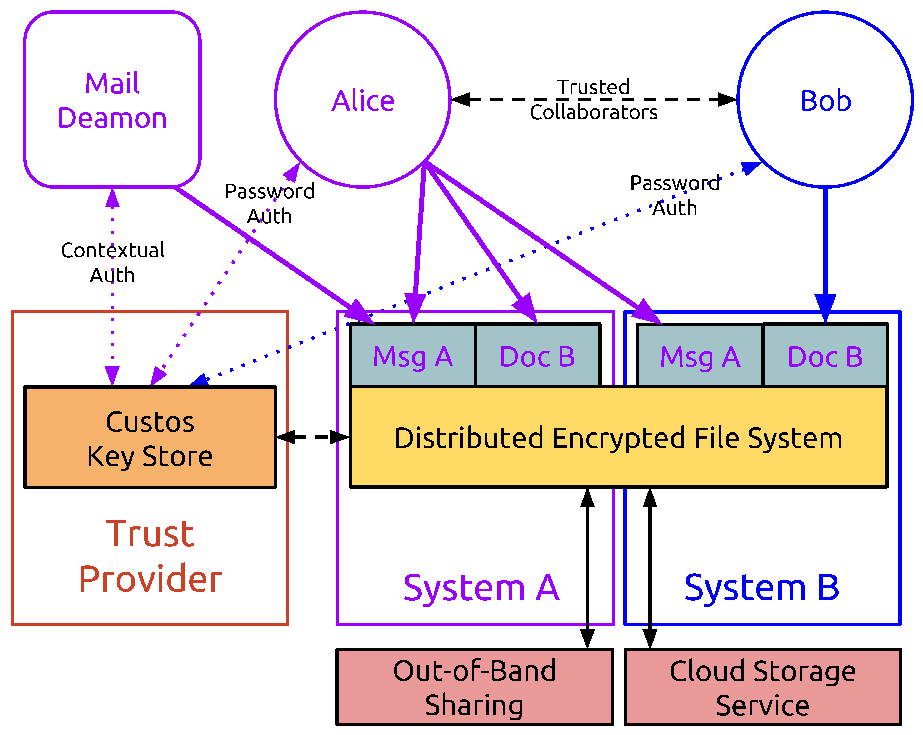
\includegraphics[width=.5\linewidth]
                        {./figs/pdf/FS-Custos-Integrated.pdf}
        \caption{Integrated File System Encryption with Custos}
        \label{fig:FS-custos-integrated}
      \end{center}
    \end{subfigure}
  \end{center}
  \caption{File System Encryption with Custos}
  \label{fig:FS-custos}
\end{figure}

Custos aims to improve upon existing encrypted file systems by
separating key storage and access control from data storage and
encryption. In doing so, Custos can support a variety of extensible
authentication mechanisms enabling a range of access control
rules. Its flexible, centralized nature also strives to simplify
multi-device syncing and multi-user sharing, as well as provide
support for a variety of modern and future use cases.

Figure \ref{fig:FS-custos-layered} shows how traditional layered files
systems (Figure \ref{fig:FS-traditional-layered}) might be improved
through incorporation with Custos. The logically centralized nature of
Custos allows Alice to now access her files on a range of devices. It
also allows her to grant access to Bod, her trusted
collaborator. Custos's support for flexible authentication schemes
including context-based authentication allows it to even support
non-interactive key access by systems like a mail daemon. In all
cases, Custos provides a single point for controlling, revoking, and
auditing access.

Figure \ref{fig:FS-custos-integrated} shows how traditional integrated
file systems (Figure \ref{fig:FS-traditional-integrated}) might be
improved through the incorporation of Custos. As in the layered case,
the Custos's centralization and flexible authentication mechanisms
allow for simple multi-user, multi-device, and non-interactive
access. In addition, mechanisms like out-of-band sharing are now
possible, since encrypted files may be moved around or stored on cloud
services without having to worry about ensuring future access to their
corresponding encryption keys. These keys are all stored in Custos,
and will be potentially available wherever the file needs to be
accessed.

\subsection{Secret Stores}

Anther possible use case for Custos is as a cloud-based secret
manager. Such a service

Limitations of Current Systems vs Flexibility w/ Custos

\subsection{Social Media}

Facebook, Google, Etc

\section{Threat Model}

\subsection{Threats}

Malevolent Custos Provider, Malevolent Client, Etc

\subsection{Mitigation}

Distributing/Sharding Trust, Etc

\subsection{Limitations}

Trade-off between 3rd party trust and flexibility
